\documentclass[fleqn]{article}

%%%%%%%%%%%%%%%%%%%%% Pre-document %%%%%%%%%%%%%%%%%%%%%
\usepackage{fancyhdr}
\usepackage{titlesec}
\usepackage{float}
\usepackage{array}
\usepackage{nicematrix}
\usepackage{multicol}
\usepackage{enumitem}
\usepackage{listings}
\usepackage{xcolor}
\usepackage{scrextend}
\usepackage{titlesec}
\usepackage{colortbl}
\usepackage{tikz}
\usetikzlibrary{shapes.geometric, arrows}

\lstdefinelanguage[RISC-V]{Assembler} {
  alsoletter={.},
  alsodigit={0x},
  morekeywords=[1]{ % instructions
    lw, sw,
    sll, slli,
    add, addi, sub,
    xor, xori, or, ori, and, andi,
    beq, bne, blt, bge, bltu, bgeu,
    j, jr, jal, jalr, ret,
  },
  morekeywords=[2]{ % registers
    x0, x1, x2, x3, x4, x5, x6, x7, x7, x8, x9, x10,
    x11, x12, x13, x14, x15, x16, x17, x18, x19, x20, 
    x21, x22, x23, x24, x25, x26, x27, x28, x29, x30, x31 },
  morecomment=[l]{;},   % mark ; as line comment start
  morecomment=[l]{\#},  % as well as #
}

\titleformat{\subsubsection}[runin]
    {\normalfont\bfseries}% formatting commands to apply to the whole heading
    {\thesubsection}% the label and number
    {0.5em}% space between label/number and subsection title
    {}% formatting commands applied just to subsection title
    []% punctuation or other commands following subsection title

% define some colors
\definecolor{pink}{rgb}{204, 0, 68}
\definecolor{blue}{rgb}{77, 148, 255}

\lstset{
  % listings sonderzeichen (for german weirdness)
  literate={ö}{{\"o}}1
           {ä}{{\"a}}1
           {ü}{{\"u}}1,
  basicstyle=\ttfamily,
  breaklines=true,
  commentstyle=\color{gray!50!black},
  keywordstyle=[1]\color{pink},
  % keywordstyle=[2]\color{blue}, 
  stringstyle=\color{mauve},                    % strings are from the telekom
  language=[RISC-V]Assembler,                   % all code is RISC-V
  tabsize=4,                                    % indent tabs with 4 spaces
  showstringspaces=false                        % do not replace spaces with weird underlines
}


\setlength{\parindent}{0pt} % Remove auto paragraph indents
\renewcommand\labelitemi{{\boldmath$\cdot$}}
\setlength{\mathindent}{0pt}  

% Get rid of those big margins
\usepackage[margin=1in]{geometry}
\newlength\titleindent
\setlength\titleindent{2cm}

\begin{document}

\pagestyle{fancy}
% Header
\fancyhead{}
\fancyhead[L]{Stephanie L'Heureux}
\fancyhead[R]{\thepage}
% No page numbers for footer
\fancyfoot{}

\begin{center}
    \Large{\textbf{Chapter 4 Exercises}}\\
\end{center}
\vspace{0.25in}

\subsubsection*{4.5} For the problems in this exercise, assume that there are no pipeline stalls and that the breakdown of the
executed instructions is as follows:

\begin{table}[H]
    \centering
    \begin{tabular}{|c|c|c|c|c|c|}
    \hline
    \rowcolor[HTML]{79bde8} 
    add & addi & not & beq & lw & sw \\ \hline \hline
    20\% & 20\% & 0\% & 25\% & 25\% & 10\% \\ \hline
    \end{tabular}
\end{table}


\subsubsection*{4.5.1 [10] \textlangle 4.3\textrangle} In what fraction of cycles is the data memory used?
\vspace{0.125in}
\begin{addmargin}[0.15cm]{0cm}
Data memory or the memory unit is a state element with inputs for addresses and the write data, 
and a single output for the read result. This part of the data path is utilized for load 
(\verb|lw|) and store (\verb|sw|) instructions. It is worth noting, the data memory is 
different than the instruction memory in the data path. In a pipelined processor, there 
will be four more cycles than the number of instructions, however as the number of 
instructions increases towards $\infty$, those four make up an negligible fraction 
of the total cycles. Therefore, the fraction of cycles in which data memory is used is: \[25\% + 10\% = 35\% \Rightarrow \frac{7}{20}\]
\end{addmargin}


\vspace{0.125in}
\subsubsection*{4.8} In this exercise, we examine how pipelining affects the clock cycle time of the processor. Problems in
this exercise assume that individual stages of the datapath have the following latencies:

\begin{table}[H]
    \centering
    \begin{tabular}{|c|c|c|c|c|}
    \hline
    \rowcolor[HTML]{79bde8} 
    IF & ID & EX & MEM & WB \\ \hline \hline
    250ps & 350ps & 150ps & 300ps & 200ps \\ \hline
    \end{tabular}
\end{table}

Also, assume that instructions executed by the processor are broken down as follows:
\begin{table}[H]
    \centering
    \begin{tabular}{|c|c|c|c|}
    \hline
    \rowcolor[HTML]{79bde8} 
    alu & beq & lw & sw  \\ \hline \hline
    45\% & 20\% & 20\% & 15\% \\ \hline
    \end{tabular}
\end{table}
\subsubsection*{4.8.1 [5] \textlangle 4.5\textrangle} What is the clock cycle time in a pipelined and non-pipelined processor?
\begin{itemize}
    \item[(a)] All pipeline stages take a single clock cycle, so the clock cycle must be long enough to accommodate the slowest operation. In this case the slowest operation is the instruction decode (ID) at 350ps. Therefore the pipelined clock cycle time is 350ps.
    \item[(b)] In a non-pipelined processor, each instruction executes after the other, one at a time. To complete one instruction, the time for each operation is added together, for the worst case instruction. \[250\text{ps} + 350\text{ps} + 150\text{ps} + 300\text{ps} + 200\text{ps} = 1250\text{ps}\] 
\end{itemize}

\subsubsection*{4.8.2 [10] \textlangle 4.5\textrangle} What is the total latency of an LW instruction in a pipelined and non-pipelined processor?
\begin{itemize}
    \item[(a)] The \verb|lw| instruction uses every stage in the execution process (IF, ID, EX, MEM and WB). For a pipelined processor, each operation takes the same amount of time, in this case $350\text{ps}$. So the total latency of the \verb|lw| instruction is $350\text{ps} \times 5 = 1750\text{ps}$
    \item[(b)] For a non-pipelined processor, stages are allowed to take different durations so in the non-pipelined example the total latency for \verb|lw| is the sum of each stage's execution time.  \[250\text{ps} + 350\text{ps} + 150\text{ps} + 300\text{ps} + 200\text{ps} = 1250\text{ps}\] 
\end{itemize}
\vspace{0.125in}

\subsubsection*{4.11} Consider the following loop:
\begin{lstlisting}
    loop:
        lw r1, 0(r1)
        and r1, r1, r2
        lw r1, 0(r1)
        lw r1, 0(r1)
        beq r1,r0, loop
\end{lstlisting}
Assume that perfect branch prediction is used (no stalls due to control hazards), that there are no delay slots,
and the pipeline has full forwarding support. Also, assume that many iterations of this loop are executed
before the loop exists.

\begin{figure}[H]
    \centering
    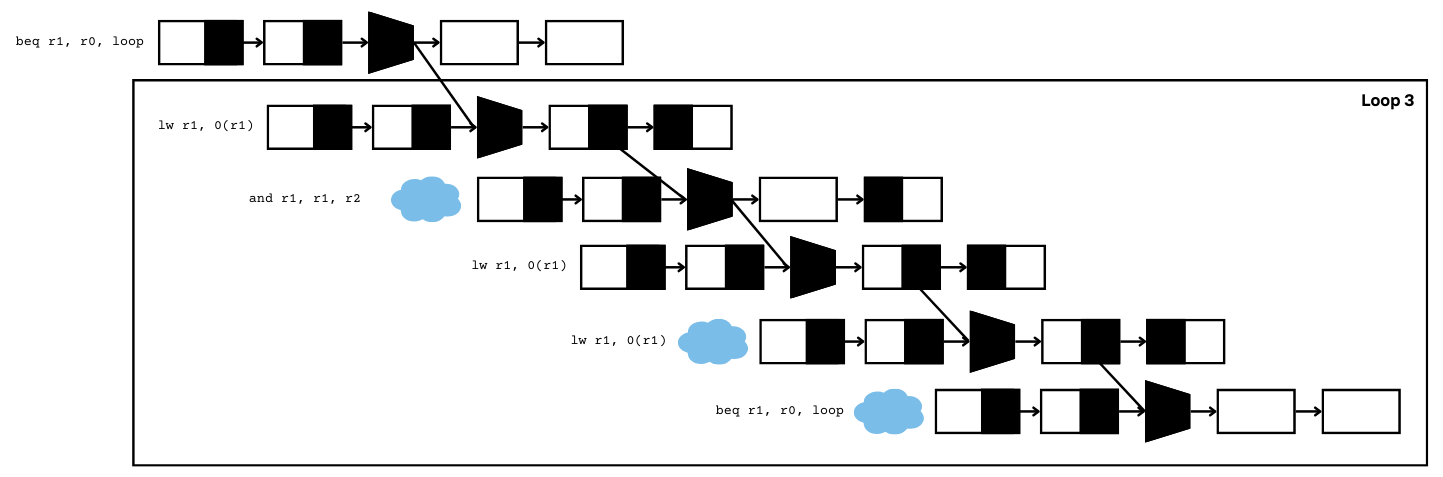
\includegraphics[width=6.5in]{p4.11.1.png}
    \caption{Pipeline for loop 3}
\end{figure}


\subsubsection*{4.11.1 [10] \textlangle 4.6\textrangle} Show a pipeline execution diagram for the third iteration of this loop, from the cycle in which we
fetch the first instruction up to (but not including) the cycle in which we can fetch the first instruction of
the next iteration. Show all instructions that are in the pipeline during these cycles (not just those from the
third iteration.
\vspace{0.125in}

\subsubsection*{4.13} This exercise is intended to help you understand the relationship between forwarding, hazard detection,
and ISA design. problems in this exercise refer to the following sequence of instructions and assume that it
is executed of a 5-stage pipelined datapath:
\begin{lstlisting}
    add r5, r2, r1
    lw r3, 4(r5)
    lw r2, 0(r2)
    or r3, r5, r3
    sw r3, 0(r5)
\end{lstlisting}


\subsubsection*{4.13.1 [5] \textlangle 4.5\textrangle} If there is no forwarding or hazard detection, insert nops to ensure correct execution.
\begin{figure}[H]
    \centering
    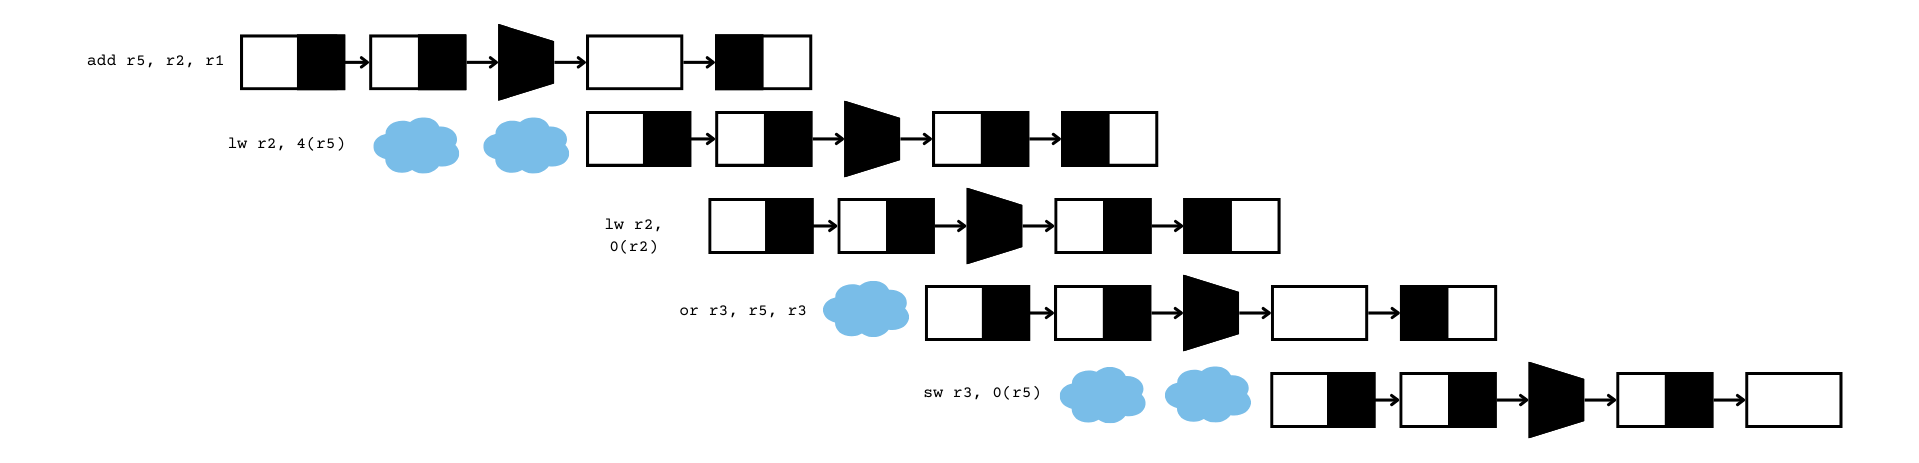
\includegraphics[width=6.5in]{p4.13.1.png}
    \caption{Pipeline with inserted nops}
\end{figure}

\subsubsection*{4.13.2 [10] \textlangle 4.5\textrangle} How many cycles in total are needed to complete those instructions (including the nops that you
inserted?) If regular forwarding is implemented, how many cycles are in the revised code in total?
\begin{itemize}
    \item[(a)] 14 cycles with nops.
    \item[(b)] 9 cycles with forwarding.
\end{itemize}
\vspace{0.125in}


\end{document} 